\begin{pastexam}[label={px:gk3-103-ds-04}]{高考三級資訊處理 103 年 第四題}
（申論；15 分）

如右的權重圖（weighted graph）共有 9 個節點（vertices）19 條邊（edges），回答下列問題：
\begin{center}
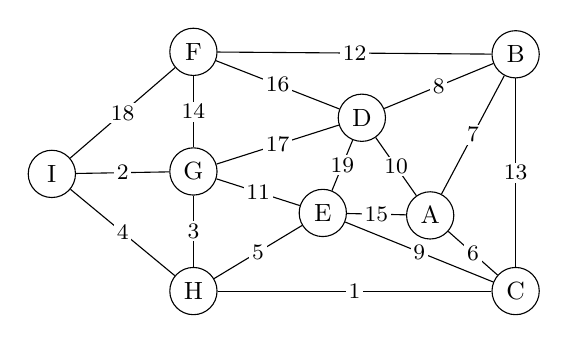
\begin{tikzpicture}[x=0.62cm, y=0.62cm,
    v/.style={circle, draw, minimum size=6mm, inner sep=0pt, font=\small},
    w/.style={fill=white, inner sep=1pt, font=\footnotesize}]
\node[v] (I) at (0.7,-3.55) {I};
\node[v] (F) at (3.6,-1.05) {F};
\node[v] (B) at (10.2,-1.1) {B};
\node[v] (D) at (7.05,-2.4) {D};
\node[v] (G) at (3.6,-3.5) {G};
\node[v] (E) at (6.25,-4.35) {E};
\node[v] (A) at (8.45,-4.4) {A};
\node[v] (H) at (3.6,-5.95) {H};
\node[v] (C) at (10.2,-5.95) {C};
\draw (F) -- node[w] {12} (B);
\draw (I) -- node[w] {18} (F);
\draw (F) -- node[w] {14} (G);
\draw (F) -- node[w] {16} (D);
\draw (D) -- node[w] {8} (B);
\draw (I) -- node[w] {2} (G);
\draw (G) -- node[w] {17} (D);
\draw (D) -- node[w] {19} (E);
\draw (D) -- node[w] {10} (A);
\draw (B) -- node[w] {7} (A);
\draw (B) -- node[w] {13} (C);
\draw (G) -- node[w] {11} (E);
\draw (E) -- node[w] {15} (A);
\draw (A) -- node[w] {6} (C);
\draw (G) -- node[w] {3} (H);
\draw (I) -- node[w] {4} (H);
\draw (H) -- node[w] {5} (E);
\draw (E) -- node[w] {9} (C);
\draw (H) -- node[w] {1} (C);
\end{tikzpicture}
\end{center}
\begin{enumerate}[leftmargin=2.2em]
\item[㈠] 請列出在運用 Kruskal's 演算法產生最小連結樹（Minimum Spanning Tree）中把邊納入最小
連結樹的順序。（3 分）
\item[㈡] 請列出運用 Prim's 演算法從 A 點開始產生最小連結樹，把邊納入最小連結樹的順序。（4 分）
\item[㈢] 設計一個 O(V)的演算法，判定在新增加一個(x,y)的邊到原圖形後，是否要更新已經產生的最小
連結樹。（8 分）
\end{enumerate}
\end{pastexam}

\begin{pastsoln}
圖上 19 條邊的權重是 1 到 19，各不相同，所以最小生成樹只有一棵（資結書定理~24.4），
Kruskal 和 Prim 選出的邊集合一定一樣，只是加入的順序不同。

\textbf{㈠ Kruskal。} 把邊由輕到重排，依序檢查：兩端已經在同一棵樹裡（加了會成環）就丟掉，
否則加入（資結書第~24.2~節）。
\begin{center}
\begin{tabular}{clll}
\toprule
權重 & 邊 & 結果 & 加入後的元件 \\
\midrule
1 & H--C & 加入 & \{H, C\} \\
2 & I--G & 加入 & \{H, C\}, \{I, G\} \\
3 & G--H & 加入 & \{C, G, H, I\} \\
4 & I--H & 丟掉（I、H 已連通） & \\
5 & H--E & 加入 & \{C, E, G, H, I\} \\
6 & A--C & 加入 & \{A, C, E, G, H, I\} \\
7 & B--A & 加入 & \{A, B, C, E, G, H, I\} \\
8 & D--B & 加入 & \{A, B, C, D, E, G, H, I\} \\
9 & E--C & 丟掉 & \\
10 & D--A & 丟掉 & \\
11 & G--E & 丟掉 & \\
12 & F--B & 加入 & 全部 9 個頂點，8 條邊，停止 \\
\bottomrule
\end{tabular}
\end{center}
加入順序：(H,C)、(I,G)、(G,H)、(H,E)、(A,C)、(A,B)、(B,D)、(B,F)，總權重
$1+2+3+5+6+7+8+12 = 44$。

\textbf{㈡ Prim，從 A 開始。} 每一步在「一端在樹裡、一端不在」的邊裡挑最輕的（資結書第~24.3~節）。
下表列出每一步時樹外各頂點目前最輕的連接邊（括號是樹裡的那一端）：
\begin{center}
\begin{tabular}{cll}
\toprule
步 & 樹外頂點的最輕連接邊 & 加入的邊 \\
\midrule
1 & B:7(A), C:6(A), D:10(A), E:15(A) & (A,C) 6 \\
2 & B:7(A), D:10(A), E:9(C), H:1(C) & (C,H) 1 \\
3 & B:7(A), D:10(A), E:5(H), G:3(H), I:4(H) & (H,G) 3 \\
4 & B:7(A), D:10(A), E:5(H), F:14(G), I:2(G) & (G,I) 2 \\
5 & B:7(A), D:10(A), E:5(H), F:14(G) & (H,E) 5 \\
6 & B:7(A), D:10(A), F:14(G) & (A,B) 7 \\
7 & D:8(B), F:12(B) & (B,D) 8 \\
8 & F:12(B) & (B,F) 12 \\
\bottomrule
\end{tabular}
\end{center}
加入順序：(A,C)、(C,H)、(H,G)、(G,I)、(H,E)、(A,B)、(B,D)、(B,F)，總權重同樣是 44。

\textbf{㈢ 新增一條邊之後要不要更新。} 設新邊是 $(x, y)$，權重 $w$，原本的最小生成樹是 $T$。
$T$ 是樹，$x$ 到 $y$ 恰好有一條簡單路徑 $P_T(x,y)$。 令 $m$ 是這條路徑上最重的邊。
\begin{itemize}
\item $w < w(m)$：把 $(x,y)$ 加進 $T$、拿掉 $m$，還是生成樹，總權重變小，所以要更新，新的
最小生成樹就是 $T - \{m\} \cup \{(x,y)\}$。
\item $w \ge w(m)$：不用更新。 原圖的其他非樹邊本來就滿足資結書定理~24.10 的條件，新邊
$(x,y)$ 也滿足 $w \ge \max_T(x,y)$，所以 $T$ 在新圖裡仍然是最小生成樹。
\end{itemize}
找路徑上最重的邊只要在 $T$ 上從 $x$ 做一次 DFS：

\begin{pseudo}{新增邊 $(x,y)$ 後是否要更新最小生成樹}
\Function{Need-Update}{$T, x, y, w$}
    \State $(\mathit{found}, m) \gets$ \Call{Max-On-Path}{$T, x, \NIL, y$}
    \If{$w < w(m)$}
        \State \Return \TRUE \Comment{用 $(x,y)$ 換掉 $m$}
    \EndIf
    \State \Return \FALSE
\EndFunction
\Statex
\Function{Max-On-Path}{$T, u, \mathit{parent}, y$} \Comment{在 $T$ 裡從 $u$ 找 $y$}
    \If{$u = y$}
        \State \Return $(\TRUE, \NIL)$
    \EndIf
    \For{$T$ 裡每條和 $u$ 相連的邊 $e = (u, v)$，$v \ne \mathit{parent}$}
        \State $(\mathit{found}, m) \gets$ \Call{Max-On-Path}{$T, v, u, y$}
        \If{$\mathit{found}$}
            \If{$m = \NIL$ \OR $w(e) > w(m)$}
                \State $m \gets e$
            \EndIf
            \State \Return $(\TRUE, m)$
        \EndIf
    \EndFor
    \State \Return $(\FALSE, \NIL)$
\EndFunction
\end{pseudo}

\proc{Max-On-Path} 回傳 $y$ 是否在 $u$ 的子樹裡，以及 $u$ 到 $y$ 這一段上最重的邊。
找到 $y$ 之後一路回傳，經過的邊就是 $x$ 到 $y$ 的路徑。 $x = y$ 時新邊是自環，$m = \NIL$，
不會被選進生成樹，這時直接回答不用更新（虛擬碼裡把 $w(\NIL)$ 當成 $-\infty$ 就好）。

\textbf{時間。} $T$ 有 $V$ 個頂點、$V-1$ 條邊，DFS 每個頂點、每條樹邊最多看一次，時間 $O(V)$。
注意只在 $T$ 上走，不在原圖上走：原圖有 $E$ 條邊，在原圖上 DFS 會是 $O(V+E)$。

以本題為例：新增 $(F, E)$ 權重 10 時，$T$ 上 F 到 E 的路徑是 F--B--A--C--H--E，最重的邊是
(B,F) 12 $> 10$，要更新，換掉 (B,F)，總權重變成 42。 新增 $(I, C)$ 權重 10 時，路徑 I--G--H--C
上最重的是 (G,H) 3 $< 10$，不用更新。
\end{pastsoln}
